\section{Performance Evaluation}
\label{sec:pe}
We present the routing performance of the proposed routing algorithm in this section.
The simulation is conducted with the dataset of the Nanjing bike sharing system,
which records the bike trips from January $1$ $2017$ to December $31$ $2017$.
Furthermore, we verify the effects of different differential privacy magnitude
on the delivery performance.

\subsection{Simulation Setup}
The simulation is implemented in Python$\footnote{\url{https://gitee.com/gaoyang23nj/DiffPrivacyOppNet}}$
and is conducted on the platform of $i5-9600K$ and $32$GB RAM.
The dataset is from the Nanjing bike sharing system,
where each bicycle trip occurs from one station to another.
We exploited the data, which ranges from June $1$ to June $30$,
to adjust the parameters before routing.
Then the proposed method is compared with the benchmarks,
e.g., Epidemic, Spary \& Wait, Prophet,
according to the trips from July $1$ to July $14$.
The size of the message is set as $10$ MB.
The source and the destination of message is chosen randomly.
The routing performance is evaluated in terms of the delivery ratio,
the average delivery latency and the communication workload.

\subsection{Generation Rate {\it v.s.}Delivery Performance}
\begin{figure*}
  \centering
  \subfloat[Delivery Ratio.]{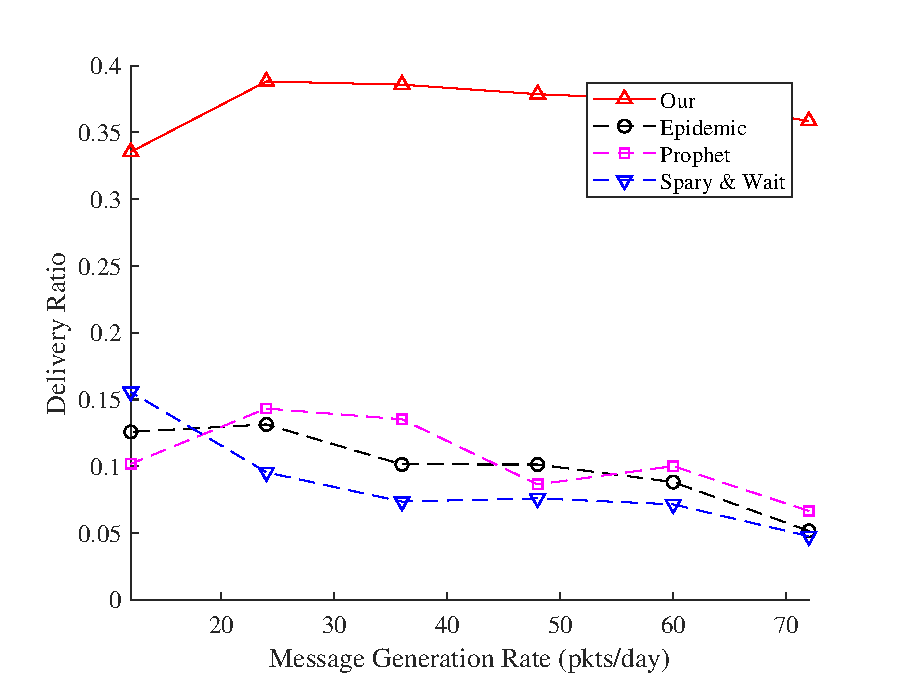
\includegraphics[width=.33\textwidth]{fig/delivery_ratio.eps}\label{fig:pe_dr}}
  \subfloat[Average Delivery Latency.]{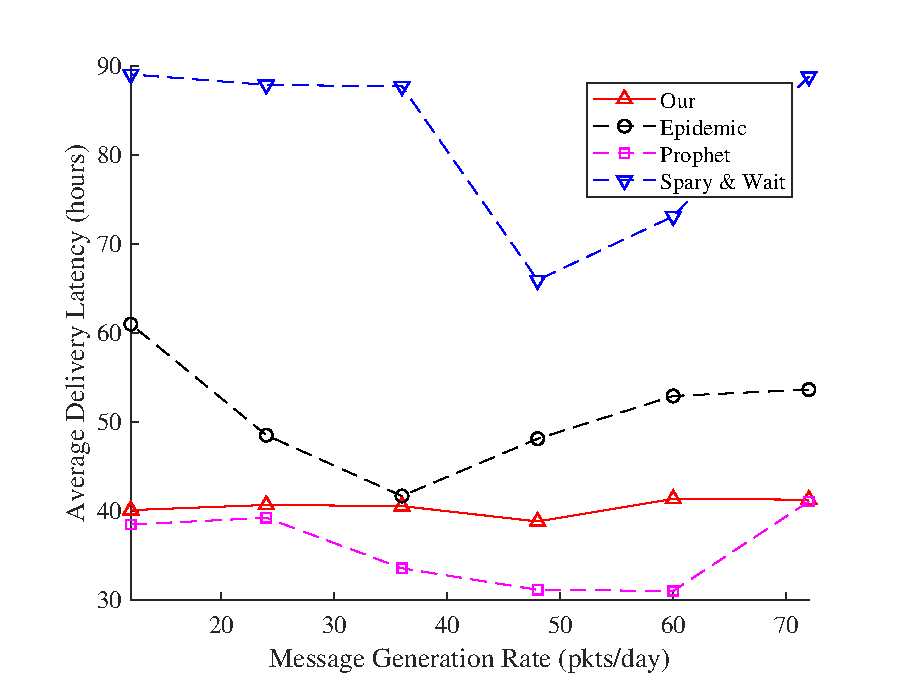
\includegraphics[width=.33\textwidth]{fig/delivery_latency.eps}\label{fig:pe_dl}}
  \subfloat[Communication Workload.]{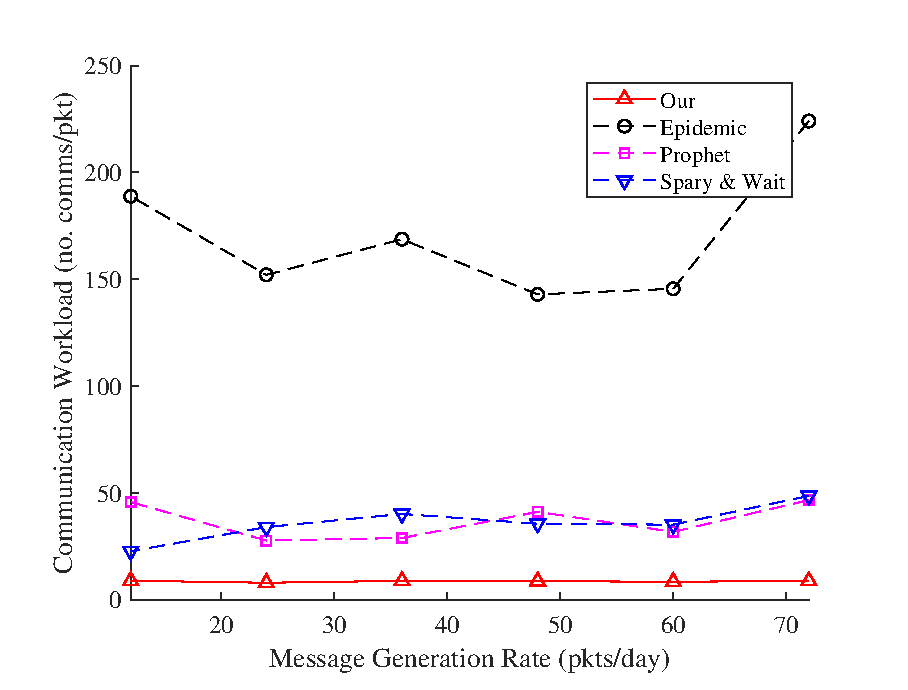
\includegraphics[width=.33\textwidth]{fig/comm_load.eps}\label{fig:pe_cl}}
  \caption{Routing Performance of different detection methods.}
  \label{fig:pe_routing}
\end{figure*}
The delivery ratios of the routing schemes are shown in Fig.~\ref{fig:pe_dr},
where the message generation rate ranges from $12$ to $72$ messages per day.
Here the lifespan of every generated message is set as $5$ days,
which means that the message that expires $5$ days will be discarded immediately.
The buffer limit of the node equals $1$ GB,
which implies that each node can carry $100$ messages in its cache.
We can find that the delivery ratio of the proposed method is about $0.4$,
which is much higher than other methods, including Epidemic, Spary \& Wait and Prophet.
This is because the two-tier probability model can estimate the probability of the future contacts
more accurately than the other methods.
Since more generated messages will induce heavier congestion,
the delivery ratios of the routing schemes decrease slightly with increasing message generation rate.

Fig.~\ref{fig:pe_dl} shows the average delivery latency of the proposed method and the benchmarks.
The Epidemic method provides the lowest delivery latency among all the methods.
This is because that the message requires longer time to be delivered is always dropped by the congestion.
Our method provides the least delivery latency except Epidemic.
The reason is that the proposed method, which takes the probabilities of multiple hops into account,
can guide the message to the proper delivery path.

The communication workload, i.e., the average number of communications,
as the main part of the energy consumption is presented in Fig.~\ref{fig:pe_cl}.
Spary \& Wait, which constrains the flooding of Epidemic via the token,
brings about $50$ communications per message,
which is much lower than Epidemic.
The communication workload of Prophet, which conducts the unicast routing,
is also similar with Spary \& Wait.
We can find that the proposed method provides the least communication workload,
which is caused by the high delivery ratio and the clear delivery path.

\subsection{Privacy Magnitude {\it v.s.} Delivery Performance}
\begin{figure*}
  \centering
  \subfloat[Delivery Ratio.]{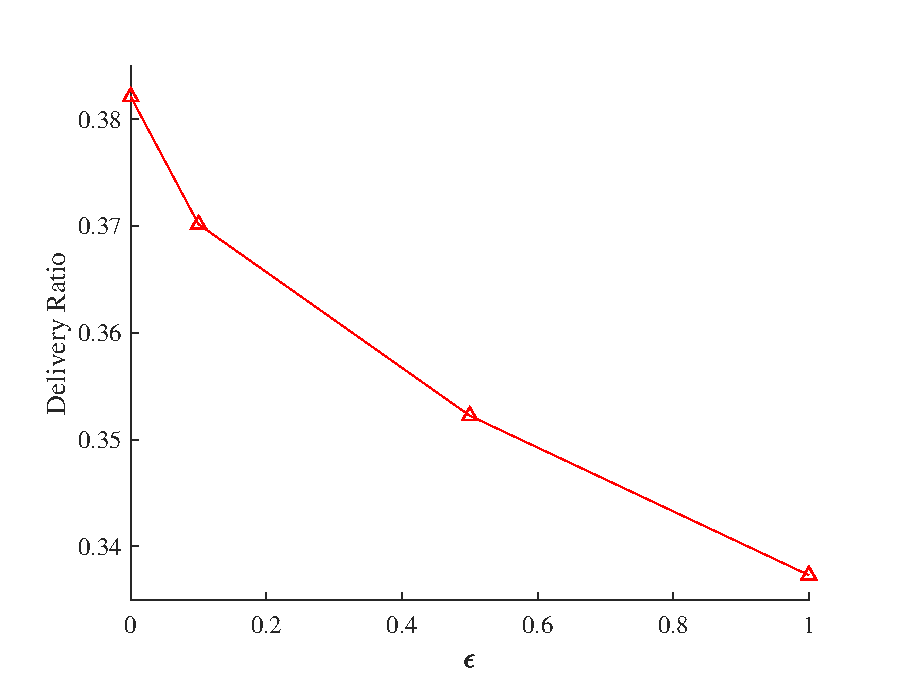
\includegraphics[width=.33\textwidth]{fig/pp_delivery_ratio.eps}\label{fig:pp_dr}}
  \subfloat[Average Delivery Latency.]{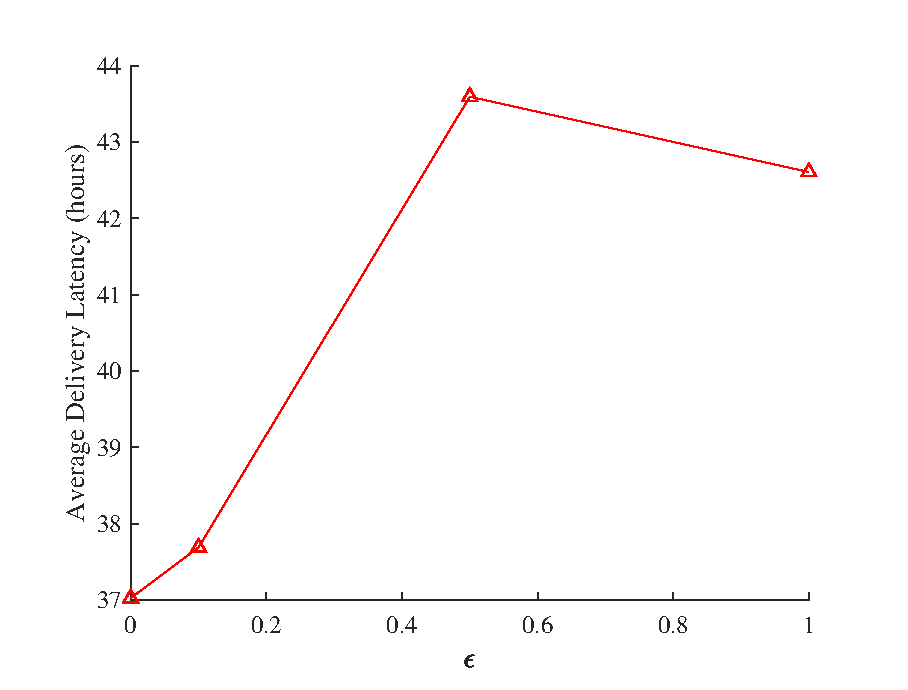
\includegraphics[width=.33\textwidth]{fig/pp_delivery_latency.eps}\label{fig:pp_dl}}
  \subfloat[Communication Workload.]{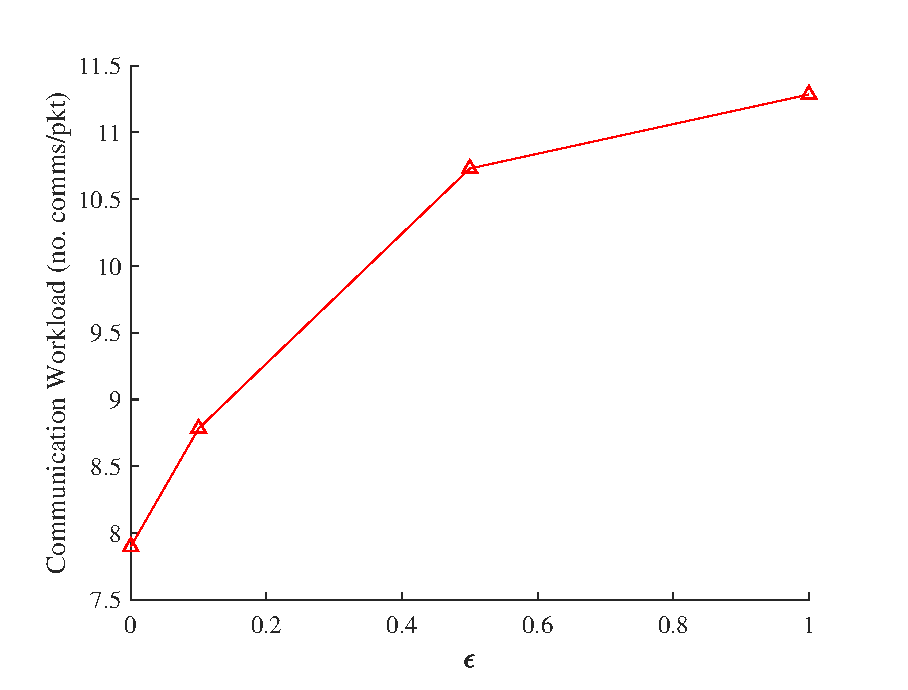
\includegraphics[width=.33\textwidth]{fig/pp_comm_load.eps}\label{fig:pp_cl}}
  \caption{Privacy Magnitude {\it v.s.} Routing Performance.}
  \label{fig:pp_routing}
\end{figure*}
The privacy magnitude also may affects the delivery performance of the proposed method.
The routing performance on the delivery ratio is presented in Fig.~\ref{fig:pp_dr}.
We can find that the delivery ratio of our proposed decreases gradually
when increasing the differential privacy magnitude of the inter-day probability $\epsilon$.
Meanwhile, we can see that the average latency and the communication workload increase
with the increasing $\epsilon$ in Fig.~\ref{fig:pp_dl} and Fig.~\ref{fig:pp_cl}.
The reason is that the probability will be published with higher noise
when higher $\epsilon$ is employed in our method.
Then the delivery metric computation will be disturbed according to $\epsilon$ and laplace mechanism.
Thus some contact with the following proper delivery path may be missed.

